\documentclass{article}
\usepackage[round]{natbib}
\usepackage{bibentry}
\usepackage{amsfonts}
\newcommand{\Rz}{\mathbb{R} }
\hyphenation{Streit-berg}
\renewcommand{\baselinestretch}{1.5}

%%\VignetteIndexEntry{Some more or less useful examples for illustration.}
%%\VignetteDepends{maxstat}


\usepackage{/usr/local/lib/R/share/texmf/Sweave}
\begin{document}

\title{Maximally Selected Rank Statistics in \textsf{R}}
\author{by Torsten Hothorn and Berthold Lausen}
\date{}

\maketitle

This document gives some examples on how to use the \texttt{maxstat} 
package and is basically an extention to \cite{on-maximal:2002}.


\section{Introduction}

The determination of two groups of observations with respect to a simple
cutpoint of a predictor is a common problem in medical statistics. For
example, the
distinction of a low and high risk group of patients is of special interest. 
The selection of a cutpoint in the predictor
%%which separates the responses best 
leads to a multiple testing problem, cf. Figure \ref{stat}. This
has to be taken into account when the effect of the selected 
cutpoint is evaluated.
Maximally selected rank statistics can be used for estimation as well as
evaluation of a simple cutpoint model. We show how this problems can be
treated with the \texttt{maxstat} package and illustrate the usage of the
package by gene expression profiling data.

\section{Maximally Selected Rank Statistics}

The functional relationship between a quantitative or ordered predictor $X$
and a quantitative, ordered or censored response $Y$ is unknown. As a simple
model one can assume that an unknown cutpoint $\mu$ in $X$ determines two
groups of observations regarding the response $Y$: 
the first group with $X$-values less or equal $\mu$
and the second group with $X$-values greater $\mu$. A measure of the
difference between two groups with respect to $\mu$ is the absolute value of
an appropriate standardized two-sample linear rank statistic of the
responses. 
We give a short overview and follow the notation in \cite{maximally-:1992}.

The hypothesis of independence of $X$ and $Y$ can be formulated as
\begin{eqnarray*}
H_0: P(Y \le y | X \le \mu) = P(Y \le y | X > \mu) \quad
\end{eqnarray*}
for all $ y $ and $ \mu \in \Rz $.
This hypothesis can be tested as follows. For every reasonable cutpoint $\mu$
in $X$
(e.g. cutpoints that provide a reasonable sample size in both groups),  the
absolute value of the standardized two-sample linear rank statistic $|S_\mu|$ 
is
computed. The maximum of the standardized statistics 
\begin{eqnarray*}
M = \max_\mu |S_\mu|
\end{eqnarray*}
of all possible
cutpoints is used as a test statistic for the hypothesis of independence
above. The cutpoint in $X$ that provides the best separation of the
responses into two groups, 
i.e. where the standardized statistics take their maximum, 
is used as an estimate of the unknown cutpoint.

Several approximations for the distribution of the maximum of the
standardized statistics $S_\mu$ have been suggested. \cite{maximally-:1992}
show that the limiting distribution is the distribution of the supremum of
the absolute value of a standardized Brownian bridge and consequently the
approximation of \cite{maximally-:1982} can be used. An approximation based
on an improved Bonferroni inequality is given by \cite{classifica:1994}. For
small sample sizes, \cite{on-the-exa:2001} derive an lower bound of the
distribution function based on the
exact distribution of simple linear rank statistics. The algorithm by
\cite{axact-dist:1986} is used for the computations.
The exact distribution
of a maximally selected Gau{\ss} statistic can be computed using the
algorithms by \cite{numerical-:1992}. Because simple linear rank statistics
are asymptotically normal, the results can be applied to approximate the
distribution of maximally
selected rank statistics \citep[see][]{on-the-exa:2001}. 

\section{The maxstat Package}

The package \texttt{maxstat} implements both cutpoint estimation and the test
procedure above with several $P$-value approximations as well as plotting
of the empirical process of the standardized statistics. It depends on the
packages \texttt{exactRankTests} for the computation of the distribution of
linear rank statistics \citep{on-exact-r:2001} and \texttt{mvtnorm} for the
computation of the multivariate normal distribution
\citep{on-multiva:2001}. The package is available at CRAN. The generic method
\texttt{maxstat.test} provides a formula interface for the specification of
predictor and response. An object of class \texttt{maxtest} is returned.
The methods \texttt{print.maxtest} and
\texttt{plot.maxtest} are available for inspectation of the results. 

\section{Gene Expression Profiling}

The distinction of two types of diffuse
large B-cell lymphoma by gene expression profiling is studied by
\cite{distinct-t:2000}. \cite{on-the-exa:2001} suggest the mean gene
expression (MGE) as quantitative factor for the discrimination between two
groups of patients with respect to overall survival time. The dataset
\texttt{DLBCL} is included in the package.
The maximally selected log-rank statistic for cutpoints between 
the $10\%$ and
$90\%$ quantile of MGE using the upper bound of the
$P$-value by \cite{on-the-exa:2001} can be computed by

\renewcommand{\baselinestretch}{1}
\begin{Schunk}
\begin{Sinput}
>library(maxstat)
\end{Sinput}
\begin{Soutput}
Loading required package: survival 
\end{Soutput}
\begin{Sinput}
>data(DLBCL)
>mtHL <- maxstat.test(Surv(time, cens) ~ MGE, data = DLBCL, 
+     smethod = "LogRank", pmethod = "HL")
\end{Sinput}
\begin{Soutput}
Loading required package: exactRankTests 
\end{Soutput}
\begin{Sinput}
>mtHL
\end{Sinput}
\begin{Soutput}
	Maximally selected LogRank statistics using HL

data:  Surv(time, cens) by MGE 
M = 3.171, p-value = 0.02218
sample estimates:
estimated cutpoint 
         0.1860526 
\end{Soutput}
\end{Schunk}
\renewcommand{\baselinestretch}{1.5}

\begin{figure}[t]
\begin{center}   
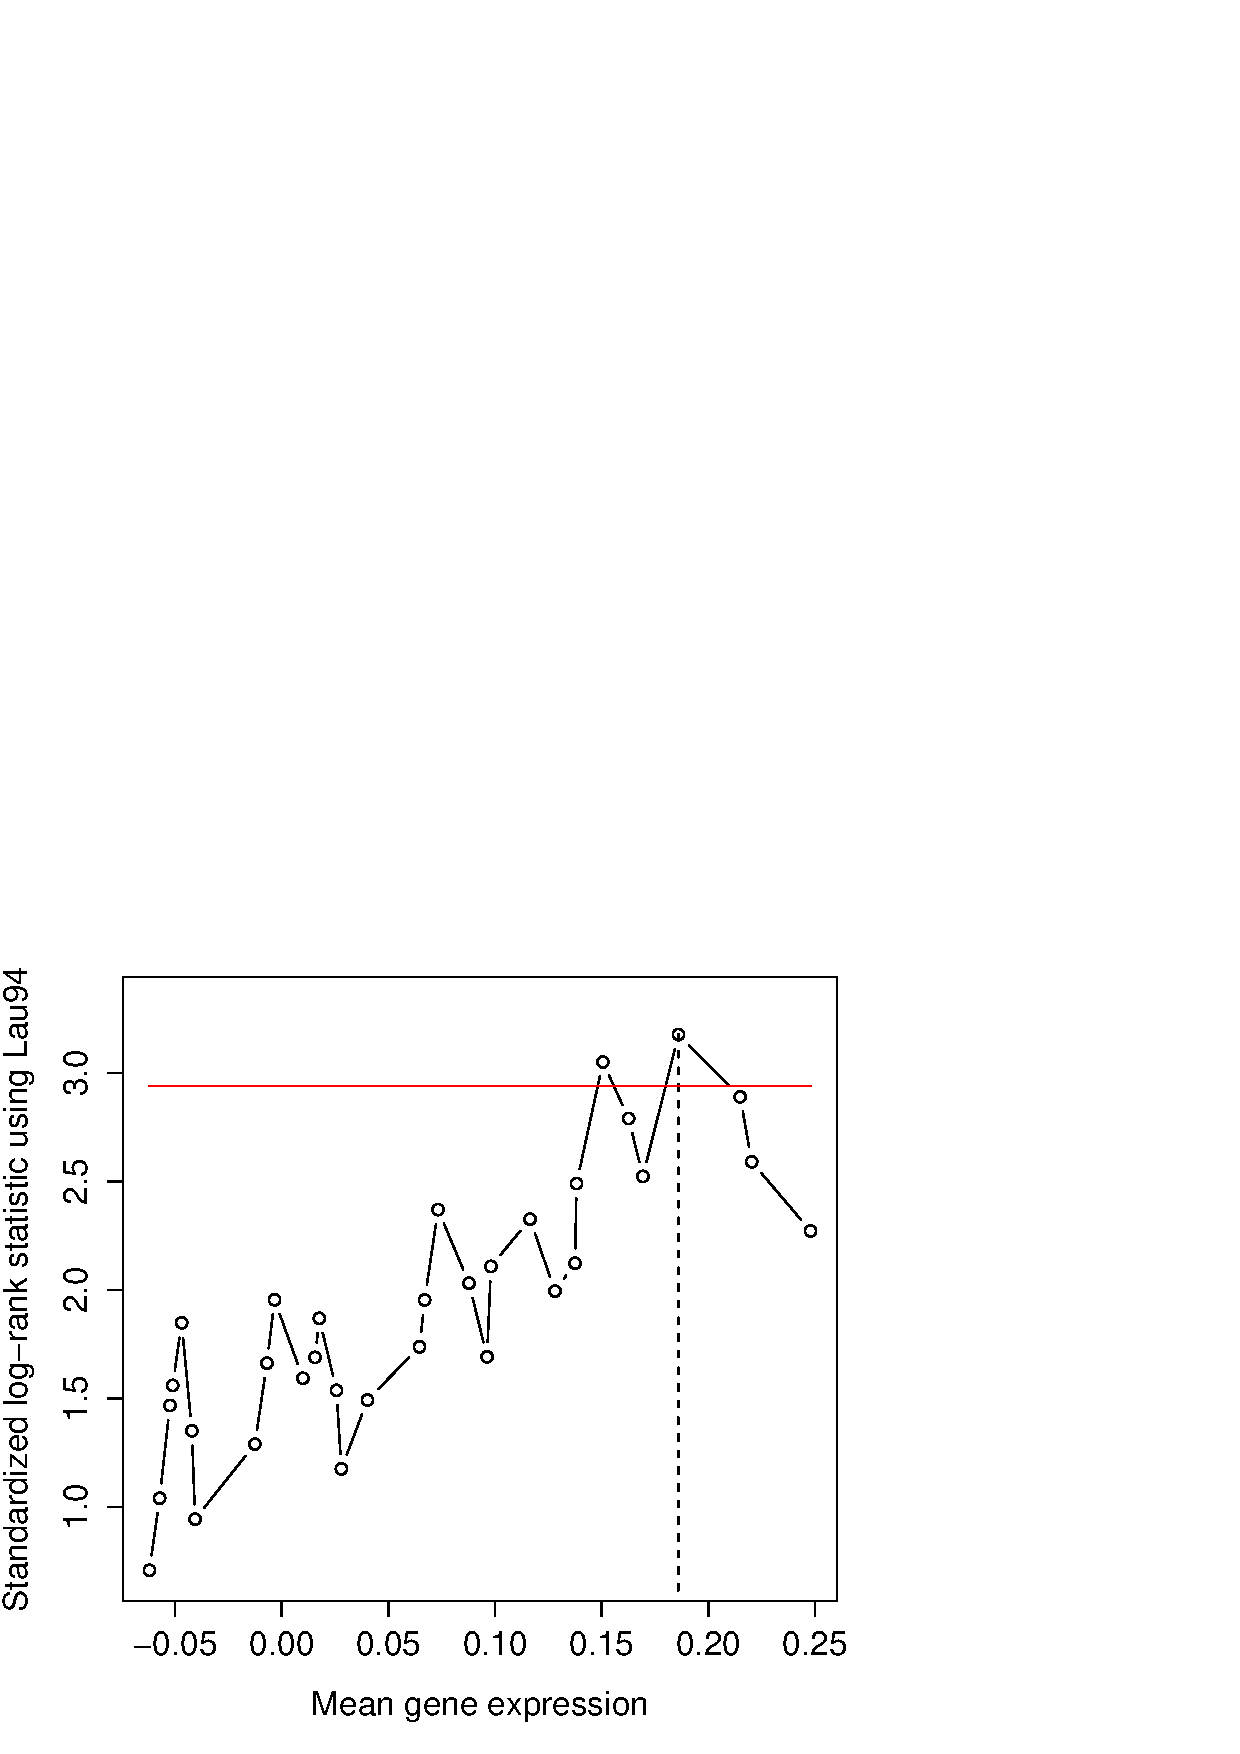
\includegraphics{maxstat-DLBCL-fig}
\caption{Absolute standardized log-rank statistics and 
significance bound based on the
improved Bonferroni inequality. \label{stat}}
\end{center}
\end{figure}

\normalsize
\renewcommand{\baselinestretch}{1.5}

For censored responses, the formula interface is similar to the one 
used in package
\texttt{survival}: \texttt{time} specifies the time until an event and
\texttt{cens} is the status indicator (\texttt{dead=1}). For quantitative
responses $y$, the formula is of the form \texttt{y} $ \sim$ \texttt{x}. 
Currently it is not possible to specify more than one predictor \texttt{x}. 
\texttt{smethod} allows the selection of the statistics to be used:
\texttt{Gauss, Wilcoxon, Median, NormalQuantil} and \texttt{LogRank} are
available.
\texttt{pmethod} defines which kind of $P$-value approximation is computed: 
\texttt{Lau92} means the
limiting distribution, \texttt{Lau94} the approximation based on the improved
Bonferroni inequality, \texttt{exactGauss} the distribution of a maximally
selected Gau{\ss} statistic and \texttt{HL} is 
the upper bound of the $P$-value by
\cite{on-the-exa:2001}. All implemented approximations are known to be
conservative and therefore their minimum $P$-value is available by choosing
\texttt{pmethod="min"}. 

\begin{figure}[t]
\begin{center}
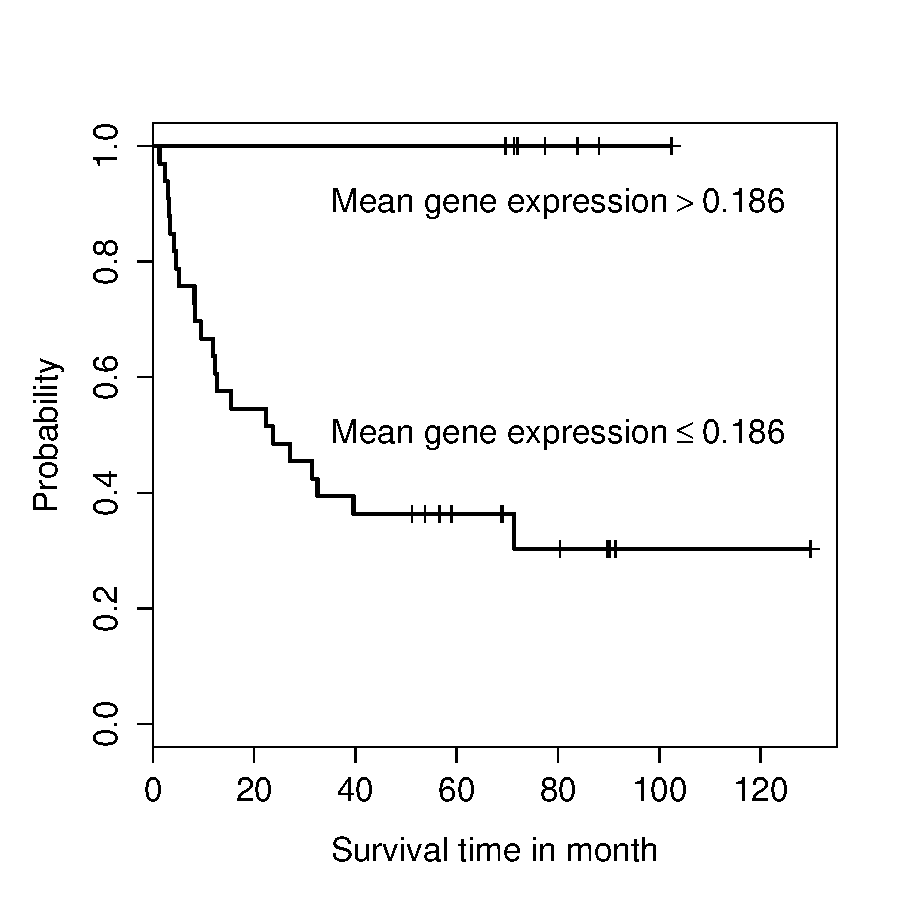
\includegraphics{maxstat-DLBCL-fig2}
\caption{Kaplan-Meier curves of two groups of DLBCL patients separated by the
cutpoint 0.186 mean gene expression. \label{surv}}
\end{center}
\end{figure}


For the overall survival time, the estimated cutpoint is
0.186 mean gene
expression, the maximum of the log-rank statistics is $M =$
3.171. The
probability that, under the null hypothesis, the maximally selected log-rank
statistic is greater $M =$
3.171 is less then than
0.022. 
The empirical process of the standardized
statistics together with the $\alpha$-quantile of the null distribution 
can be plotted using \texttt{plot.maxtest}. 
If the significance level \texttt{alpha} is specified, 
the corresponding quantile is computed and drawn
as a horizonal red line. 
The estimated cutpoint is plotted as vertical dashed line, see Figure
\ref{stat}. 
The difference in overall survival time between the two groups determined by
a cutpoint of 0.186 mean gene expression is plotted in Figure
\ref{surv}. No event was observed for patients with mean gene expression
greater 0.186.

The exact conditional $p$-value can be simulated via conditional
Monte-Carlo. This may be time consuming but is an easy way to check the goodness of
the $p$-value approximations. The argument \texttt{B} specifies
the number of Monte-Carlo replications to be performed (and defaults to
$10000$).

\begin{Schunk}
\begin{Sinput}
>maxstat.test(Surv(time, cens) ~ MGE, data = DLBCL, 
+     smethod = "LogRank", pmethod = "condMC", B = 9999)
\end{Sinput}
\begin{Soutput}
	Maximally selected LogRank statistics using condMC

data:  Surv(time, cens) by MGE 
M = 3.1772, p-value = 0.0122
sample estimates:
estimated cutpoint 
         0.1860526 
\end{Soutput}
\end{Schunk}



\section{More than One Predictor}

If the cutpoints in more than one predictor are evalutated, the problem is
to test the null hypothesis of independence of the response and any of the
predictors under consideration. Furthermore, the ``best'' split in the
``most significant'' predictor needs to be selected. For example, we
evaluate both mean gene expression and the International Prognostic Index
(IPI) simultaneously:

\renewcommand{\baselinestretch}{1}
\begin{Schunk}
\begin{Sinput}
>mmax <- maxstat.test(Surv(time, cens) ~ MGE + 
+     IPI, data = DLBCL, smethod = "LogRank", pmethod = "exactGauss", 
+     abseps = 0.01)
\end{Sinput}
\begin{Soutput}
Loading required package: mvtnorm 
\end{Soutput}
\begin{Sinput}
>mmax
\end{Sinput}
\begin{Soutput}
	 Optimally Selected Prognostic Factors 

Call: maxstat.test.data.frame(formula = Surv(time, cens) ~ MGE + IPI, 
    data = DLBCL, smethod = "LogRank", pmethod = "exactGauss", 
    abseps = 0.01)


 Selected: 

	Maximally selected LogRank statistics using
	exactGauss

data:  Surv(time, cens) by IPI 
M = 2.9603, p-value = 0.01148
sample estimates:
estimated cutpoint 
                 1 

Adjusted p.value: 
0.03088528 , error:  0.007842964 
\end{Soutput}
\end{Schunk}
\renewcommand{\baselinestretch}{1.5}

The p-value of the global test for the null hypothesis ``survival is
independent from both IPI and MGE'' is 0.031 
and IPI provides a better distinction into two groups than 
MGE does. We can display the
standardized statistics using \texttt{plot} (Figure \ref{plotmmax}). The
methodology used here is described in \cite{lausenetal:2002}.

\begin{figure}[ht]
\begin{center}
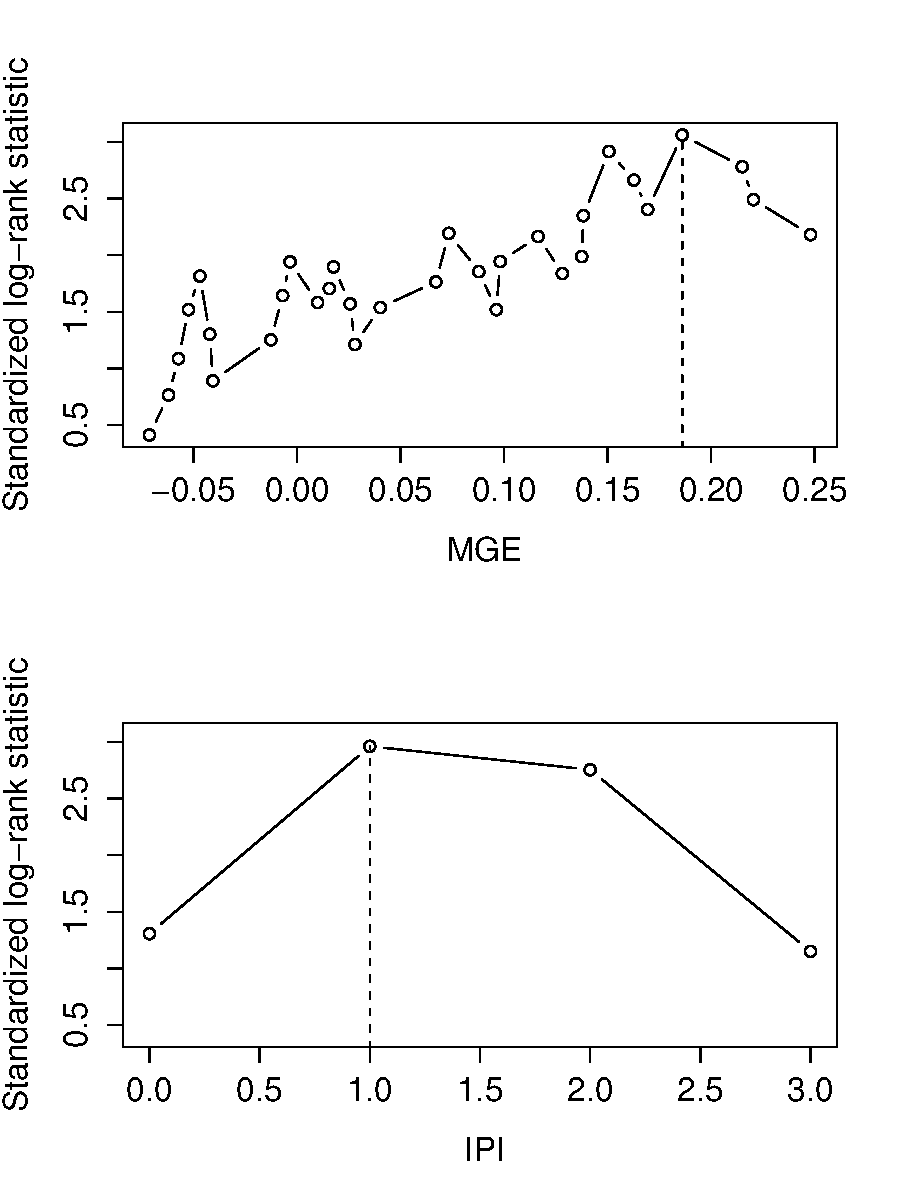
\includegraphics{maxstat-mmax-fig}
\caption{The standardized logrank statistics for the two predictors MGE and
IPI. \label{plotmmax}}
\end{center}
\end{figure}

\section{Summary}

The package \texttt{maxstat} provides a user-friendly interface and 
implements standard methods as well as recent suggestions for the 
approximation of the null distribution of maximally selected rank statistics.


\bibliographystyle{plainnat}
\bibliography{maxstatlit}

\end{document}
